\documentclass{ximera}
%herschreven 2 september 2026
\title{Het elektrisch veld}
\author{Daan Lipkens}

\begin{document}
\begin{abstract}
    De definitie van het elektrisch veld.
\end{abstract}
\maketitle

%\section{Het concept van een elektrisch veld}

We zeggen dat er een \textbf{elektrisch veld} bestaat in de ruimte rondom een geladen voorwerp (de \textit{bronlading}). Wanneer een ander geladen voorwerp (de \textit{testlading}) in dit veld wordt geplaatst, zal het veld een elektrische kracht uitoefenen op deze testlading, zoals te zien op figuur~\ref{fig:testlading_bronlading}.

\begin{definition}[title={Het Elektrisch Veld}]\nl
    De elektrische veldvector $\vec{E}$ in een bepaald punt in de ruimte is gedefinieerd als de elektrische kracht $\vec{F}_e$ die inwerkt op een positieve testlading $Q_t$ in dat punt, gedeeld door de grootte van die testlading:
    $$ \vec{E} = \frac{\vec{F}_e}{Q_t} $$
    De SI-eenheid van het elektrisch veld is de \textbf{newton per coulomb (N/C)}.
\end{definition}

%---------------------------
% AFBEELDING: Figuur 23.10 (Testlading bij bronlading)
\begin{figure}[ht!]
    \captionsetup{width=0.85\textwidth}
    \begin{center}
        
\includegraphics[height=8cm,width=12cm, keepaspectratio]{pic5/elektriciteit/veld/testlading_bronlading.png}
        % TIP: Gebruik hier de afbeelding van Figure 23.10 uit het boek
    \end{center}
    \caption{Een kleine positieve testlading $Q_t$ geplaatst in de buurt van een grotere positieve bronlading $Q$ ondervindt een elektrisch veld $\vec{E}$.}
    \label{fig:testlading_bronlading}
\end{figure}
%---------------------------

%---------------------------
% ANALOGIE ZWAARTEKRACHT
\begin{remark}[expandable, title={Analogie met het zwaarteveld}]\nl
    De definitie van het elektrisch veld lijkt heel sterk op iets wat we al kennen: het zwaarteveld! %Als veldkracht, een kracht dat geen contact nodig heeft om een invloed uit te oefenen, is er een bijhorend veld. Denk terug aan de zwaartekracht en het zwaarteveld.
    Net zoals een voorwerp met massa $m$ een zwaartekracht $\vec{F}_g$ ondervindt in het zwaarteveld $\vec{g}$ van de aarde, ondervindt een lading $Q_t$ een elektrische kracht $\vec{F}_e$ in een elektrisch veld $\vec{E}$.
    
    \begin{itemize}
        \item \textbf{Zwaarteveld:} $\vec{g} = \frac{\vec{F}_g}{m} \implies \vec{F}_g = m\cdot\vec{g}$
        \item \textbf{Elektrisch veld:} $\vec{E} = \frac{\vec{F}_e}{Q_t} \implies \vec{F}_e = Q_t\cdot\vec{E}$
    \end{itemize}

    \begin{center}
        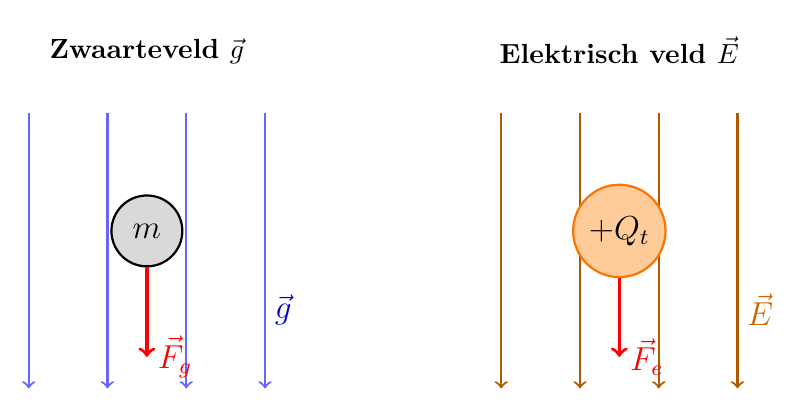
\begin{tikzpicture}[scale=1]
            % --- ZWAARTEVELD (Links) ---
            \node[above, font=\bfseries] at (0, 2) {Zwaarteveld $\vec{g}$};
            
            % Veldlijnen g (blauw)
            \foreach \x in {-1.5, -0.5, 0.5, 1.5} {
                \draw[->, thick, blue!60] (\x, 1.5) -- (\x, -2);
            }
            \node[blue!80!black, right, font=\large] at (1.5, -1) {$\vec{g}$};
            
            % Massa
            \node[circle, draw=black, fill=gray!30, thick, minimum size=9mm, font=\large] (m) at (0,0) {$m$};
            
            % Zwaartekracht
            \draw[->, very thick, red] (m) -- (0,-1.6) node[right, font=\large] {$\vec{F}_g$};

            % --- ELEKTRISCH VELD (Rechts) ---
            \node[above, font=\bfseries] at (6, 2) {Elektrisch veld $\vec{E}$};
            
            % Veldlijnen E (oranje)
            \foreach \x in {4.5, 5.5, 6.5, 7.5} {
                \draw[->, thick, orange!70!black] (\x, 1.5) -- (\x, -2);
            }
            \node[orange!80!black, right, font=\large] at (7.5, -1) {$\vec{E}$};
            
            % Lading
            \node[circle, draw=orange!90!red, fill=orange!40, thick, minimum size=9mm, font=\large] (q) at (6,0) {$+Q_t$};
            
            % Elektrische kracht
            \draw[->, very thick, red] (q) -- (6,-1.6) node[right, font=\large] {$\vec{F}_e$};
        \end{tikzpicture}
    \end{center}
\end{remark}
%---------------------------

\begin{proposition}[foldable=true,title={Eigenschappen van het elektrisch veld}]\nl
    \begin{itemize}
        \item Het veld $\vec{E}$ wordt gecreëerd door de bronlading(en), \textbf{niet} door de testlading zelf\footnote{De testlading zelf maakt ook een elektrisch veld, maar heeft geen invloed in dat punt zelf.}.
        \item Het veld bestaat in de ruimte rondom de bronlading, ongeacht of er effectief een testlading aanwezig is om het veld te detecteren.
        \item Als we de formule omvormen, kunnen we de kracht op elke willekeurige lading $Q$ in een gekend veld eenvoudig berekenen via $\vec{F}_e = Q\cdot \vec{E}$. Bij een positieve lading wijzen de kracht en het veld in dezelfde richting. Bij een negatieve lading wijzen ze in tegengestelde zin.
    \end{itemize}
\end{proposition}


\begin{proposition}[foldable=true,title={Elektrische kracht op een lading in een elektrisch veld}]\nl
    De grootte van de kracht die op een lading $Q$ inwerkt in een elektrisch veld $E$ wordt gegeven door $F=Q\cdot E$. De richting van deze kracht is steeds evenwijdig met het elektrisch veld (zie figuur~\ref{fig:kracht_lading_in_veld}). De zin hangt af van het teken van de lading: bij een \textbf{positieve} lading heeft de kracht dezelfde zin als het elektrisch veld. Bij een \textbf{negatieve} lading is de zin van de kracht net \textbf{tegengesteld} aan die van het elektrisch veld.
    %---------------------------------
% FIGUUR: kracht op lading in homogeen veld
\begin{center}
    \centering
    \begin{tikzpicture}[scale=1]
        % ----- PANEEL (a): positieve lading -----
        \begin{scope}
            % homogeen veld: evenwijdige veldlijnen naar rechts
            \foreach \y in {0, 1.2, 2.4}{
                \draw[vector] (0,\y) -- (3.4,\y);
            }
            \node[above] at (1.7,2.5) {$\vec{E}$};

            % lading tussen twee veldlijnen (geen overlap met de pijlen)
            \coordinate (Qpos) at (1.4,0.6);
            \draw[charge+] (Qpos) circle (2*\R) node[scale=1.3] {$+$};

            % kracht: zelfde zin als het veld
            \draw[force] (Qpos) ++ (2*\R+0.1,0) -- ++(1.1,0) node[right] {$\vec{F}$};

            \node[below] at (1.7,-0.5) {(a) positieve lading};
        \end{scope}

        % ----- PANEEL (b): negatieve lading -----
        \begin{scope}[xshift=6cm]
            \foreach \y in {0, 1.2, 2.4}{
                \draw[vector] (0,\y) -- (3.4,\y);
            }
            \node[above] at (1.7,2.5) {$\vec{E}$};

            \coordinate (Qneg) at (2.0,0.6);
            \draw[charge-] (Qneg) circle (2*\R) node[scale=1.3] {$-$};

            % kracht: tegengestelde zin aan het veld
            \draw[force] (Qneg) ++ (-2*\R-0.1,0) -- ++(-1.1,0) node[left] {$\vec{F}$};

            \node[below] at (1.7,-0.5) {(b) negatieve lading};
        \end{scope}
    \end{tikzpicture}
    \captionof{figure}{De kracht op een lading in een homogeen elektrisch veld. (a) Op een positieve lading werkt de kracht in dezelfde zin als het veld. (b) Op een negatieve lading werkt de kracht in de tegengestelde zin.}
    \label{fig:kracht_lading_in_veld}
\end{center}
%---------------------------------

\end{proposition}

\end{document}